% ----------------------------------------------------------
\chapter{Painéis de Monitoramento Operacional (Grafana)}
\label{ap:paineis_grafana}
% ----------------------------------------------------------

Este apêndice reúne os painéis operacionais complementares desenvolvidos na plataforma Grafana para o monitoramento contínuo de telemetria das redes sem fio do campus do ICEA/UFOP. Esses painéis serviram como ferramenta de suporte à infraestrutura durante a coleta dos dados.

\section{Painéis do Ecossistema Ruckus Wireless}

\begin{figure}[H]
	\centering
	\begin{subfigure}[b]{0.48\textwidth}
		\centering
		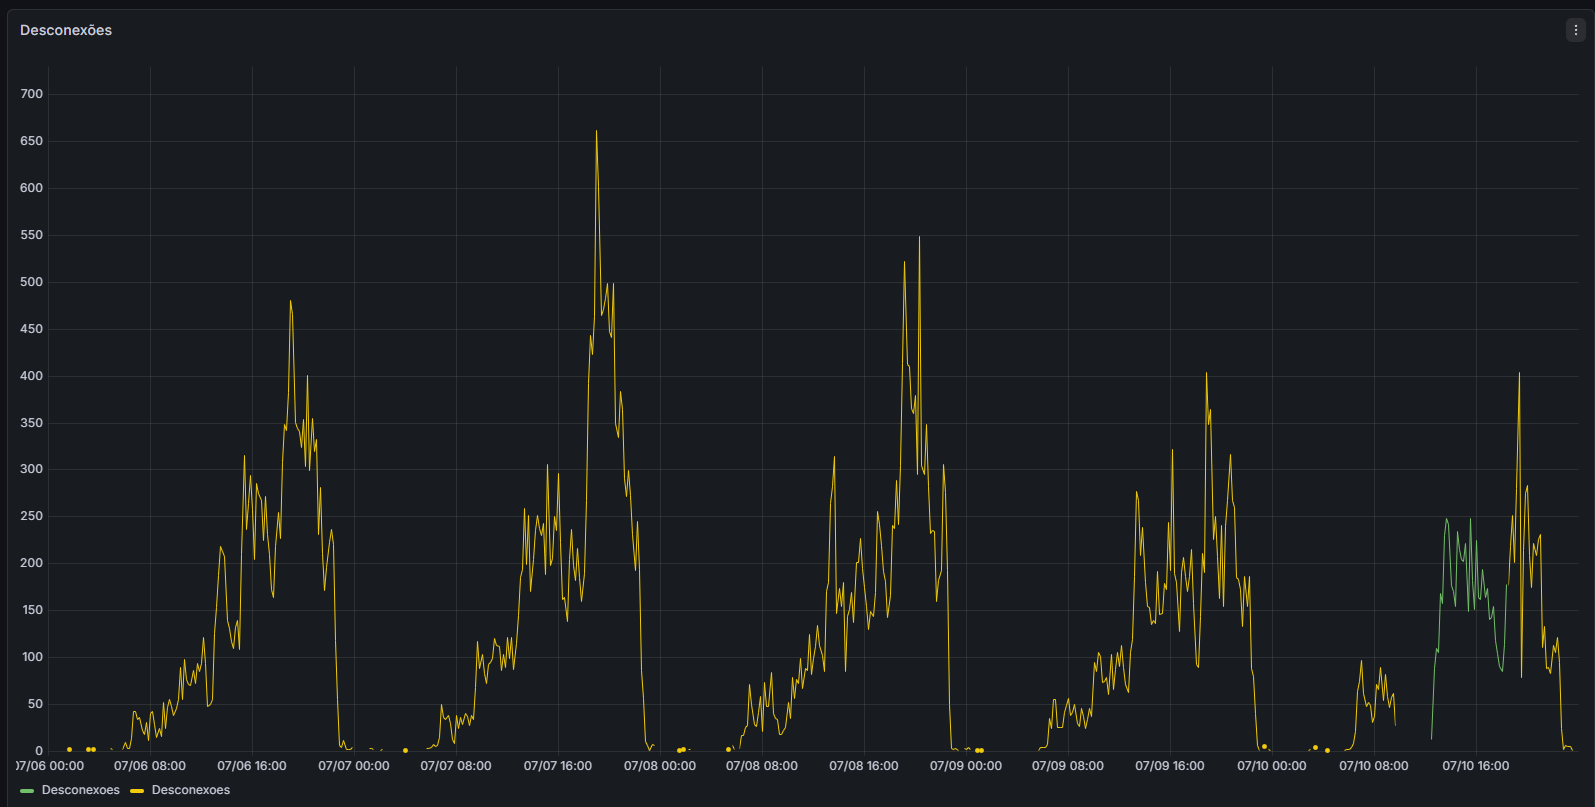
\includegraphics[width=\textwidth]{img/grafana-ruckus-desconexoes.png}
		\caption{Histórico de desconexões de clientes}
		\label{fig:ap_ruckus_desc}
	\end{subfigure}
	\hfill
	\begin{subfigure}[b]{0.48\textwidth}
		\centering
		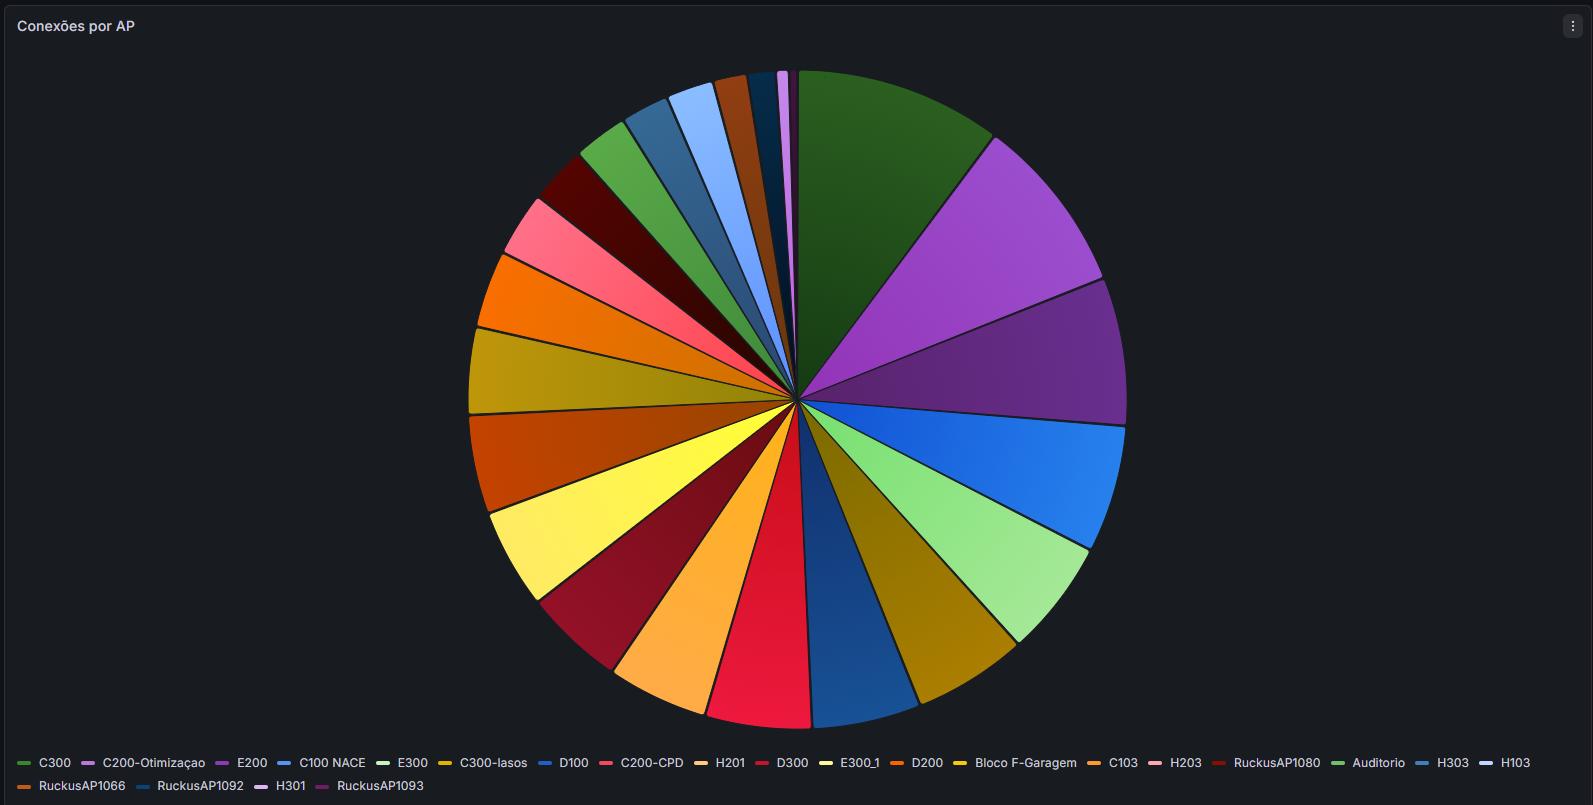
\includegraphics[width=\textwidth]{img/grafana-ruckus-con-aps.png}
		\caption{Distribuição percentual de conexões por AP}
		\label{fig:ap_ruckus_pie}
	\end{subfigure}
	\caption{Painéis do Grafana para histórico de desconexões e distribuição de clientes por AP (Ruckus)}
	\label{fig:ap_grafana_ruckus_detalhes}
	\fonte{Produzido pelos autores (2026).}
\end{figure}

\begin{figure}[H]
	\centering
	\begin{subfigure}[b]{0.48\textwidth}
		\centering
		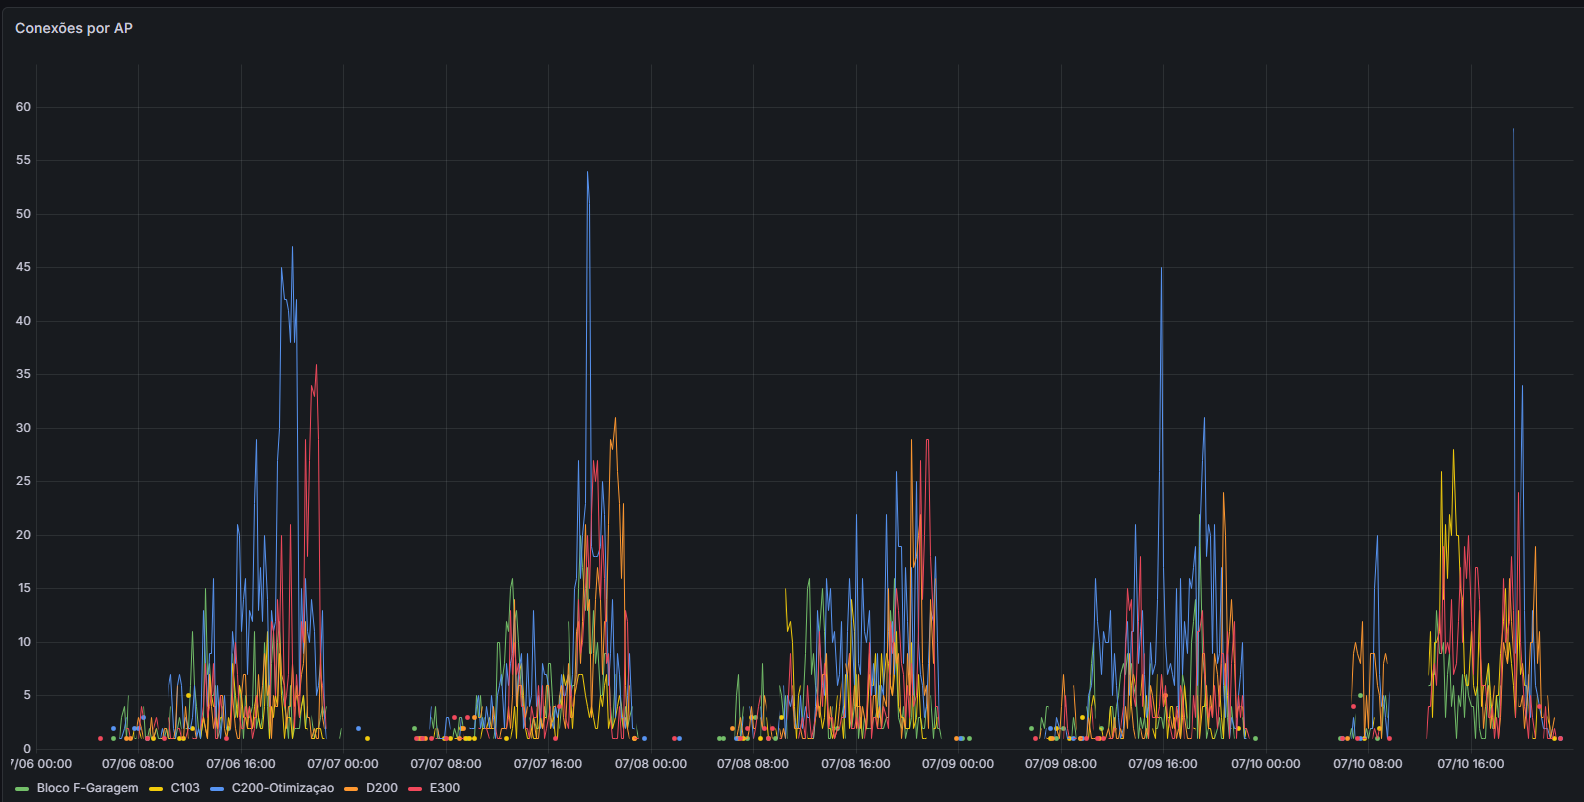
\includegraphics[width=\textwidth]{img/grafana-ruckus-con-aps-2.png}
		\caption{Linha temporal de carga por rádio}
		\label{fig:ap_ruckus_timeline}
	\end{subfigure}
	\hfill
	\begin{subfigure}[b]{0.48\textwidth}
		\centering
		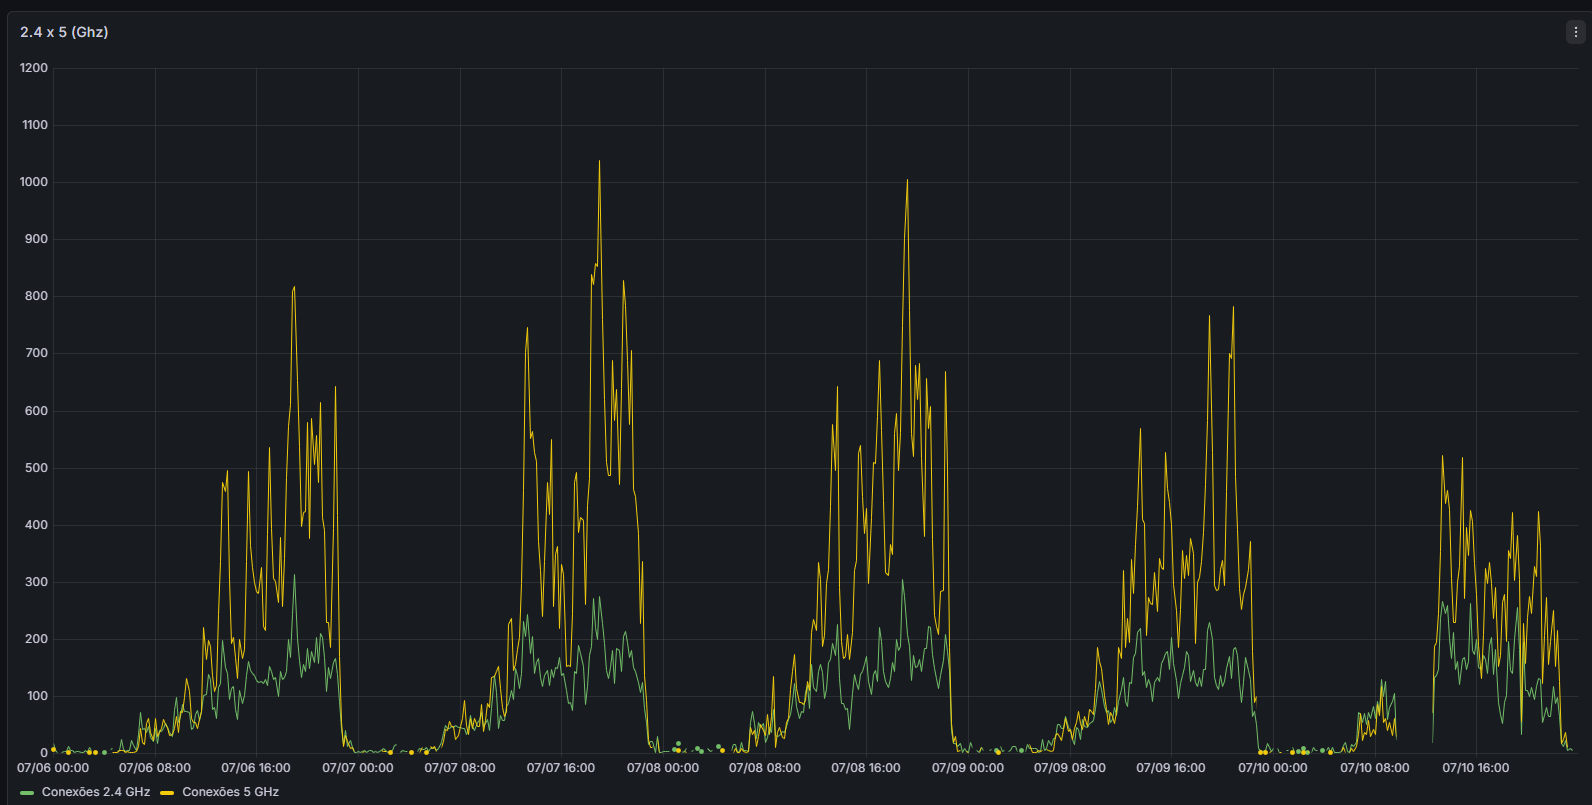
\includegraphics[width=\textwidth]{img/grafana-ruckus-2-5.png}
		\caption{Divisão de clientes por banda (2,4 GHz vs 5 GHz)}
		\label{fig:ap_ruckus_bands}
	\end{subfigure}
	\caption{Painéis do Grafana para evolução temporal e distribuição espectral de rádios (Ruckus)}
	\label{fig:ap_grafana_ruckus_tempo_bandas}
	\fonte{Produzido pelos autores (2026).}
\end{figure}

\begin{figure}[H]
	\centering
	\begin{subfigure}[b]{0.48\textwidth}
		\centering
		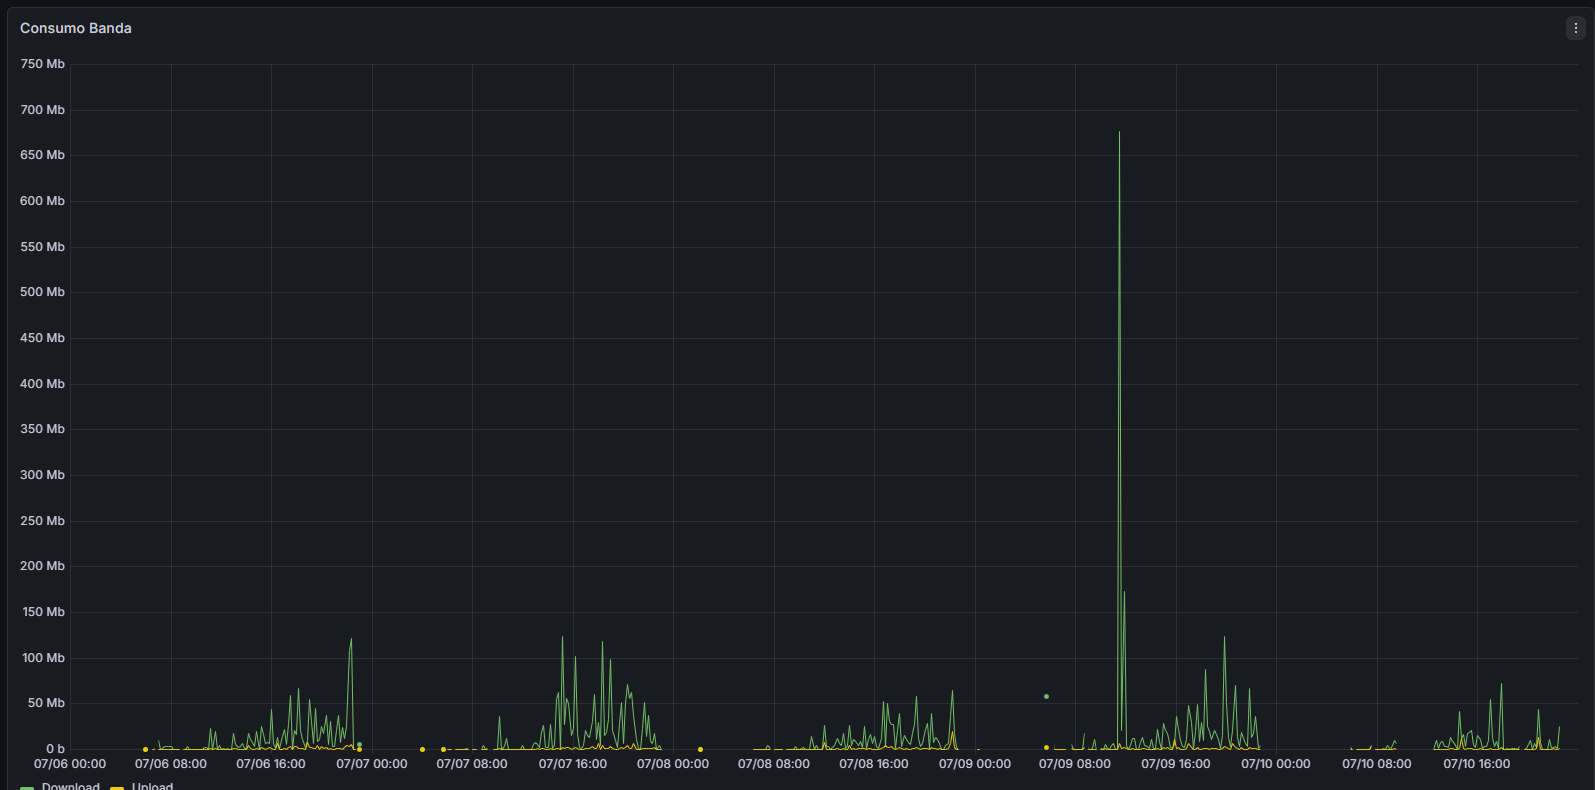
\includegraphics[width=\textwidth]{img/grafana-ruckus-banda.png}
		\caption{Throughput médio transmitido por frequência}
		\label{fig:ap_ruckus_tp_band}
	\end{subfigure}
	\hfill
	\begin{subfigure}[b]{0.48\textwidth}
		\centering
		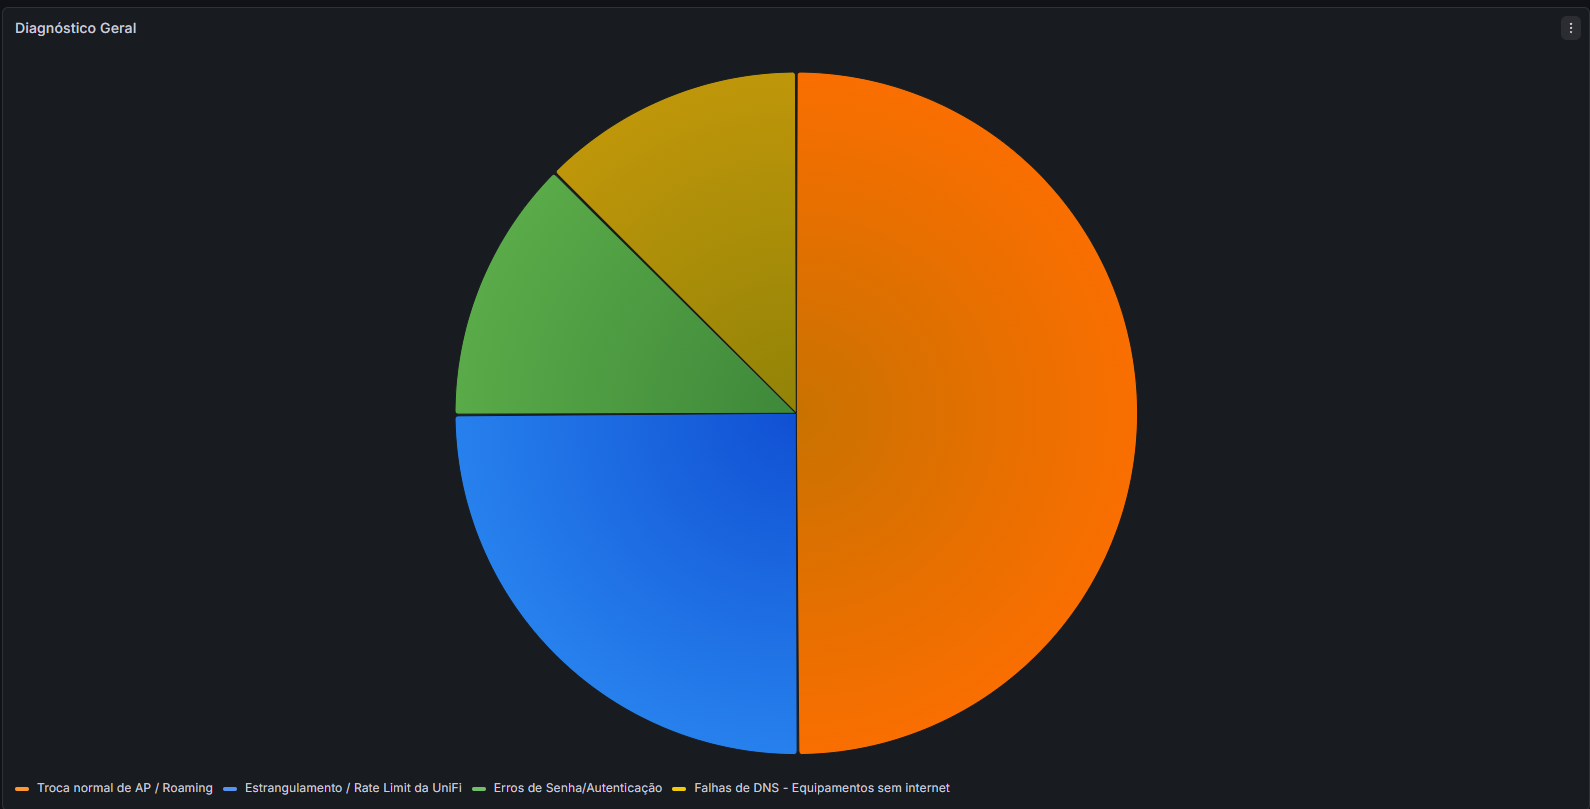
\includegraphics[width=\textwidth]{img/grafana-ruckus-diagnostico.png}
		\caption{Painel geral de diagnóstico de canais e alarmes}
		\label{fig:ap_ruckus_diag}
	\end{subfigure}
	\caption{Painéis do Grafana para throughput por frequência e diagnósticos operacionais (Ruckus)}
	\label{fig:ap_grafana_ruckus_operacional}
	\fonte{Produzido pelos autores (2026).}
\end{figure}

\section{Painéis do Ecossistema Ubiquiti UniFi}

\begin{figure}[H]
	\centering
	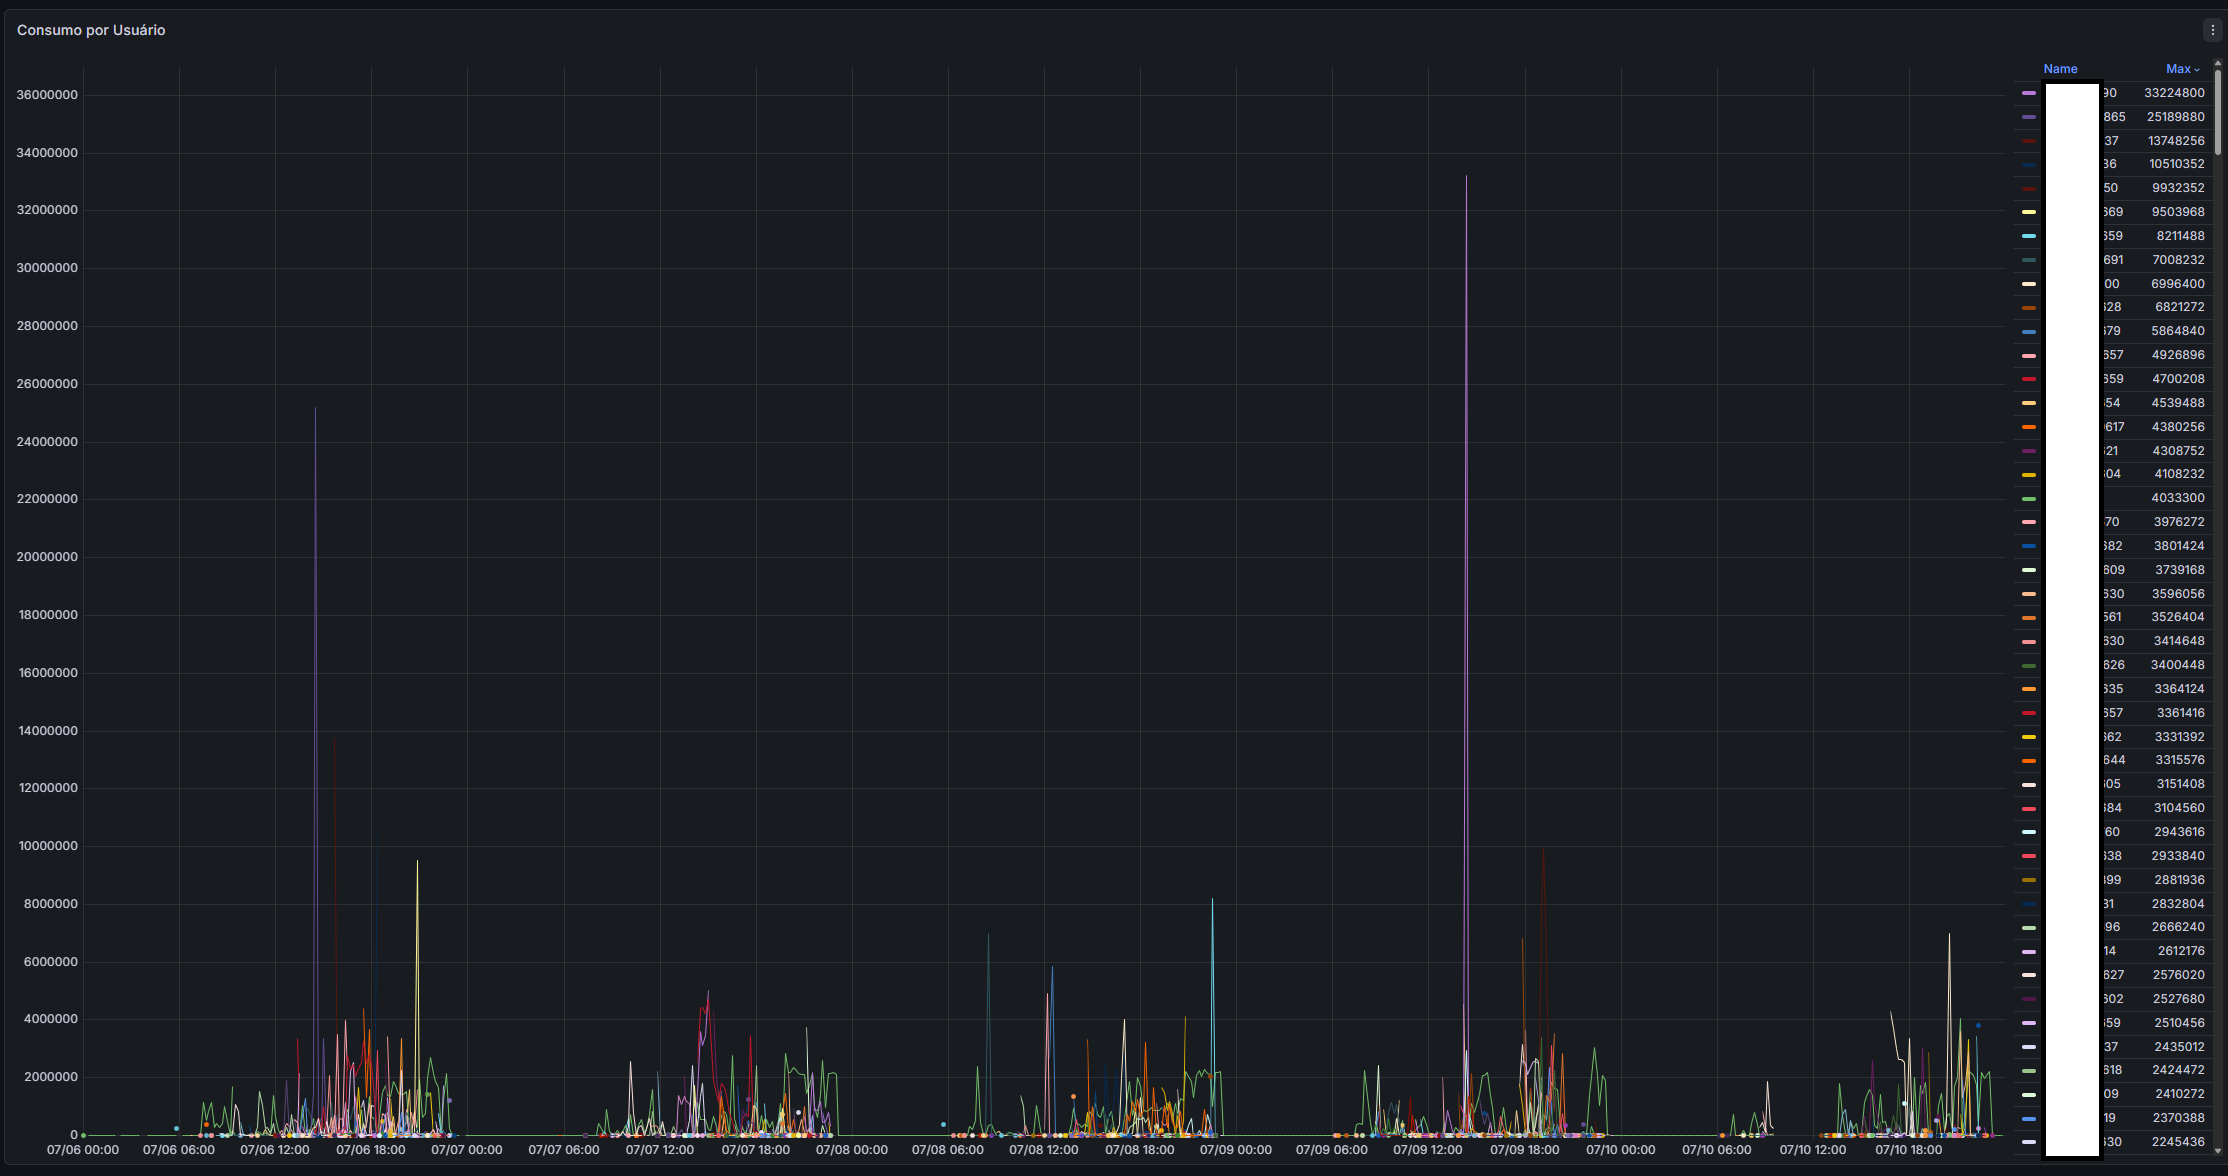
\includegraphics[width=0.85\textwidth]{img/grafana-unifi-consumo-usu.png}
	\caption{Painel do Grafana para consumo acumulado de tráfego por usuário (UniFi)}
	\label{fig:ap_grafana_unifi_consumo}
	\fonte{Produzido pelos autores (2026).}
\end{figure}
